\documentclass{article}
\usepackage{amsmath,amssymb,amsthm}
\usepackage[margin=0.5in]{geometry}
\usepackage{amsmath}
\usepackage{mathtools}  
\usepackage{multicol}
\usepackage{pdfpages}
\usepackage{indentfirst} 
\setlength{\parindent}{4em}
\setlength{\parskip}{1em}
\usepackage{relsize}
\usepackage[utf8]{inputenc}
\usepackage{float}

\title{EP4 - MAP2210 NUSP9896604}
\author{Pedro Blöss Braga}
\date{July 2020}

\begin{document}

\maketitle

\hfill

\hfill


\begin{center}
{\huge Aplicações e implementação da 
Decomposição de Valores Singulares (SVD),
e relações com Análise de Componentes Principais (PCA) }    
\end{center}

\pagebreak

\tableofcontents


\pagebreak

\section{Introdução}

\hfill

Neste texto pretendo abordar a teoria o método de decomposição de valores (Singular Value Decomposition), conhecido como SVD; sua relação forte com o método de decomposição em compontentes principais (Principal Component Analysis), PCA; expor algumas aplicações interessantes destes métodos; Fazer testes de comparação entre métodos.


\pagebreak

\section{Decomposição em Valores Singulares (SVD)}

\hfill

Este método pode ser utilizado para decompor matrizes complexas, separando a matriz original em duas matrizes unitárias e uma retangular diagonal, de valores singulares:

\begin{equation}
\mathlarger{
X = \mathcal{U} \Sigma V^T
}
\end{equation}


Caso trabalhando com uma matriz $X$ real, as matrizes $\mathcal{U}$ e $\Sigma$ também serão reais, e as conjugadas transpostas serão então simplesmente as transpostas.

\begin{equation}
\mathlarger{
\forall x_{ij} \in \mathbb{R} \Rightarrow u_{ij}, v_{ij} \in \mathbb{R}, \forall u_{ij} \in \mathcal{U}, v_{ij} \in V \Rightarrow \bar{X}^T = X^T
}
\end{equation}

\hfill

\begin{figure}[H]
\begin{center}
  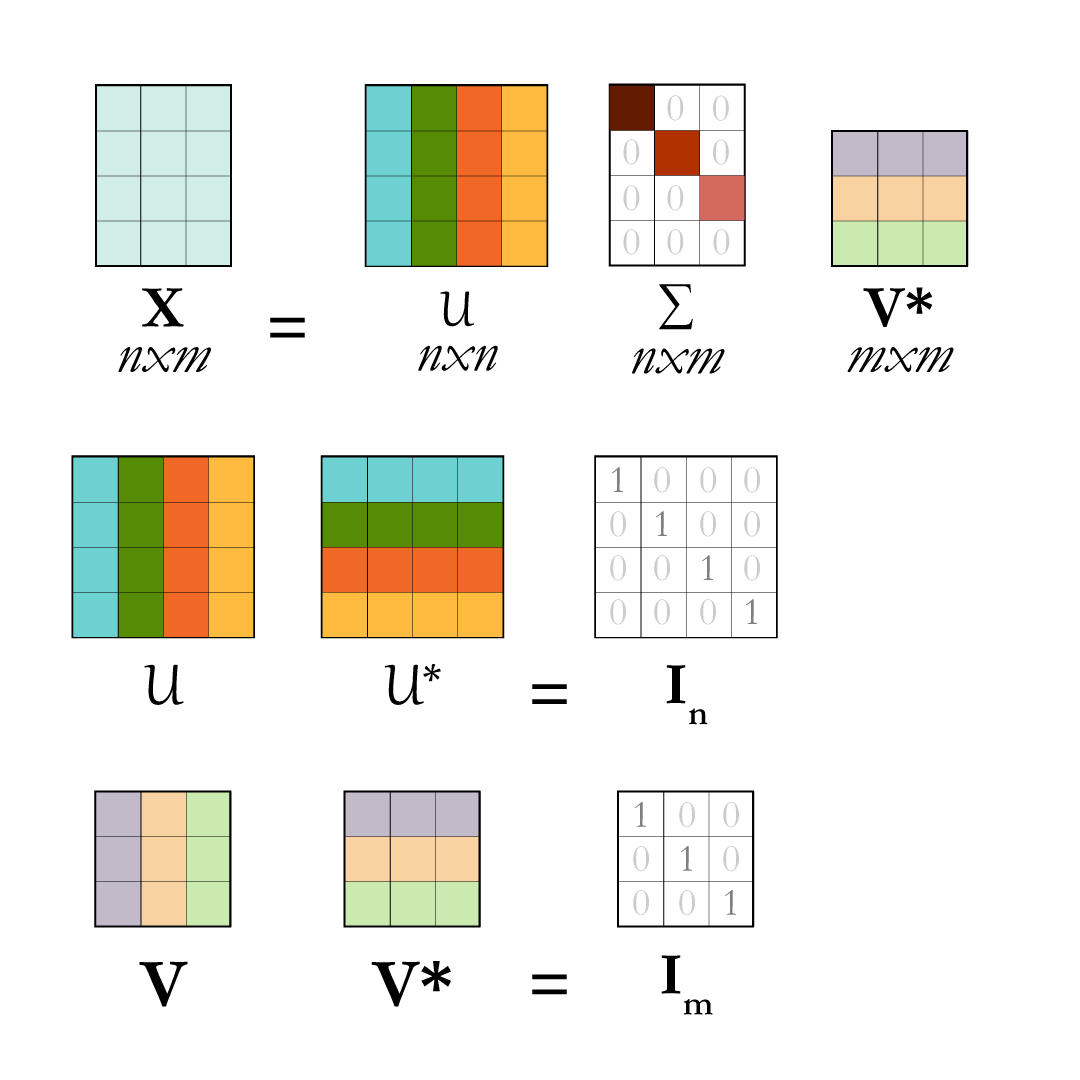
\includegraphics[width=0.4\linewidth]{images/algelin1.png}
\end{center}
\end{figure}

\hfill

Exemplo, com a matriz:

\begin{equation}
    \mathlarger{
    \begin{pmatrix}
    -10 & -10 \\
    -10 & 20 \\
    20 & 20 \\
    20 & -10 
    \end{pmatrix}
    }
\end{equation}
\begin{figure}[H]
\begin{center}
  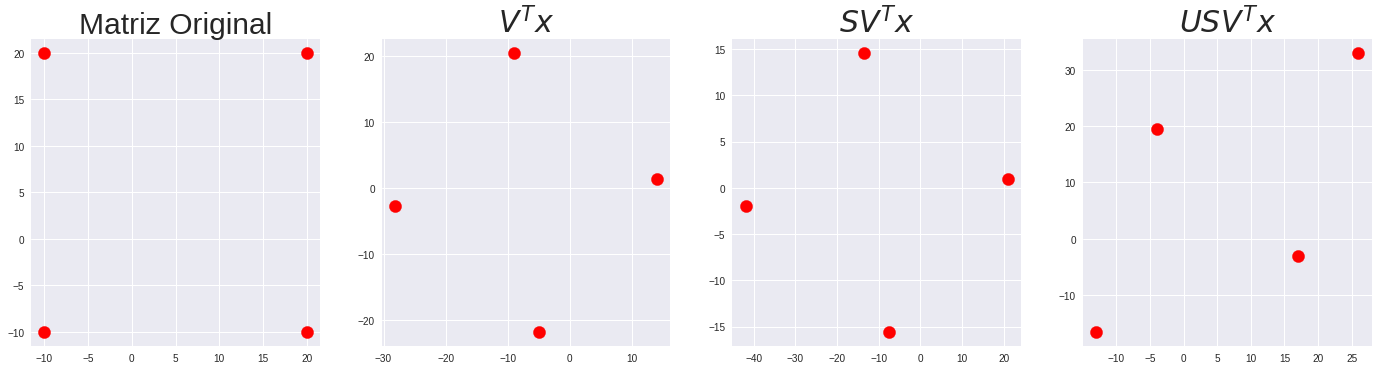
\includegraphics[width=0.6\linewidth]{images/svd_plots.png}
\end{center}
\end{figure}


\pagebreak

\section{Interpretação Geométrica do SVD}

\hfill

Ainda com a matriz bidimensional
\begin{equation}
    \mathlarger{
    X = \begin{pmatrix}
    -10 & -10 \\
    -10 & 20 \\
    20 & 20 \\
    20 & -10 
    \end{pmatrix}
    }
\end{equation}

visualizaremos as transformações, geometricamente.

$\mathbf{V^Tx}$

Podemos ver que multiplicar por $V^T$ aplica uma transformação e uma rotação à matriz de input $X$

\begin{figure}[!ht]
\begin{center}
  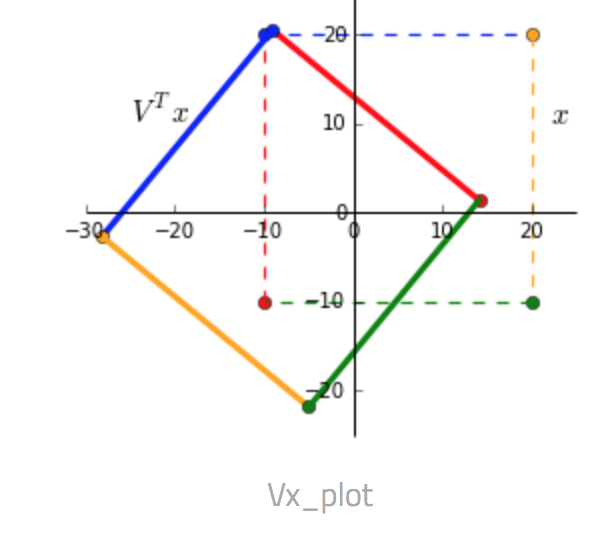
\includegraphics[width=0.4\linewidth]{images/Vx_plot.png}
\end{center}
\end{figure}

$\mathbf{SV^Tx}$

Agora, com $S$, a matriz passa a levar em conta valores na diagonal, escalando a matriz (multiplicando por algum valor).

$V$ rotaciona a matriz para uma posição em que os valores singulares representam o fator de escalamento sobre a base V.
(Na foto, $V^TX$ está tracejado e $SV^T X$ está em linhas sólidas).

\begin{figure}[!ht]
\begin{center}
  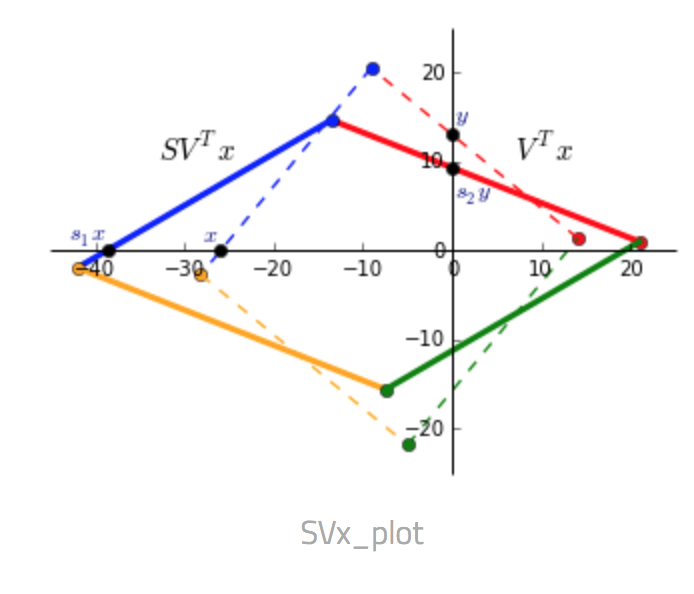
\includegraphics[width=0.4\linewidth]{images/SVx_plot.png}
\end{center}
\end{figure}

$\mathbf{USV^Tx}$

Por fim, $U$ rotaciona e reflete a matriz de volta à base inicial.

\begin{figure}[!ht]
\begin{center}
  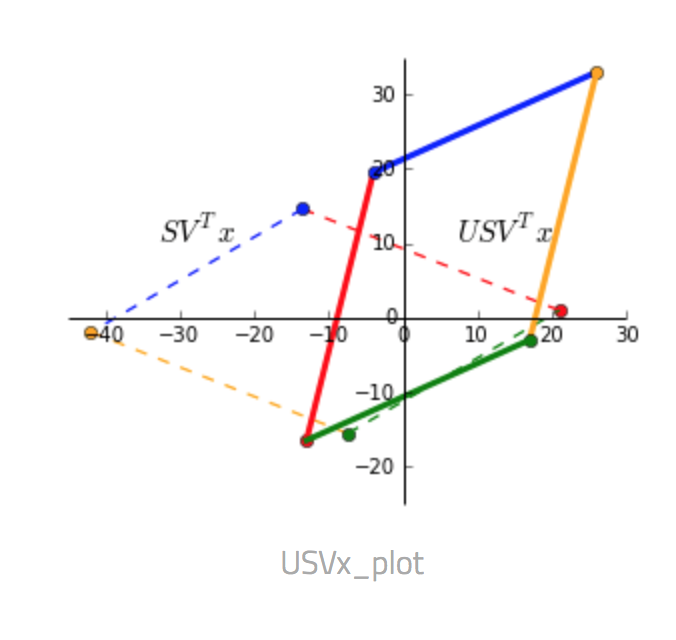
\includegraphics[width=0.4\linewidth]{images/USVx_plot.png}
\end{center}
\end{figure}

Demonstrando todos os passos em uma única imagem, obtemos:

\begin{figure}[!ht]
\begin{center}
  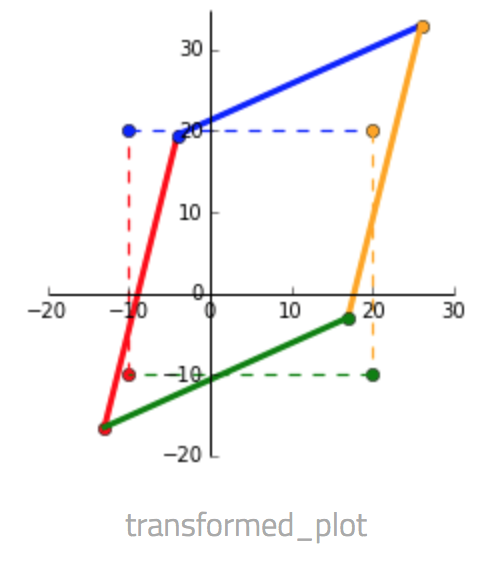
\includegraphics[width=0.4\linewidth]{images/transformed_plot.png}
\end{center}
\end{figure}

Podemos ver que os eixos no novo espaço são ortogonais. Então, os atributos originais são expressos em termos de novos atributos independentes entre si.

(Isso pode ter relação com a matriz de covariância, que expôe a independência entre componentes).


\pagebreak

\section{Análise de Componentes Principais (PCA)}

\hfill

Este método expõe eixos ortogonais não-correlacionados, denominados componentes principais (PC)s, no espaço $n$ dimensional.

Os primeiros componentes capturam os dados de maior variância.

Já que os PCs são ortogonais entre si, i.e. $\langle PC_i, PC_j \rangle = 0, i \neq j$, um par de linhas perpendiculares no $\mathbb{R}^2$ podem forma dois PCs.

O primeiro PC, que captura a maior variância, é que melhor se ajusta aos dados, linearmente. Podemos pensar que é uma reta ajustada linear, $Y = \beta_0 + \beta_1X + \epsilon$, que minimiza $\sum_i \epsilon^2$.

Os componentes principais podem ser obtidos pela decomposição da matriz de covariância:
\begin{equation}
\mathlarger{
C = W \Lambda W^{-1}
}
\end{equation}

Geometricamente, esta decomposição encontra um novo sistema de coordenadas de autovetores de $C$ por meio de rotações.

$W$ é a matriz $n$x$n$ de autovetores, e $\Lambda$ é a matriz diagonal de $n$ autovetores.

Os autovetores, que são os vetores coluna de $W$, são os PCs que procuramos.

Para obter os dados no espaço dos PCs, fazemos:
\begin{equation}
\mathlarger{
X_{k} = X W_k
}
\end{equation}

\pagebreak

\section{Relação do SVD com o PCA}

\hfill

Ambos são métodos de decomposição de matrizes retangulares.

Podemos ver, pela decomposição SVD da matriz de covariância:

\begin{equation}
\mathlarger{
C = \frac{\langle X, X \rangle}{n-1} = \frac{ V \Sigma \mathcal{U}^T U \Sigma^T V^T}{n-1} = V \frac{\Sigma^2}{n-1} V^T = V \frac{\Sigma^2}{n-1} V^{-1}
}
\end{equation}

Então, 

\begin{equation}
\mathlarger{
\Lambda = \frac{\Sigma^2}{n-1}
}
\end{equation}

Pela decomposição de autovetores de $C$, podemos verificar que os autovalores serão a matriz $\Lambda$.


\pagebreak


\section{Redução de Dimensionalidade}

\hfill

Uma matriz de dados pode descrever o comportamento de algum fator com múltiplos valores, como por exemplo um vetor de preços de algum ativo da bolsa de valores, associado a um vetor de texto podem ser input para algum modelo preditivo. 

Contudo, por vezes, gostaríamos de ter um número reduzido e compactado de informações, a fim de "explicar"
algum comportamento de alguma maneira mais "simples". Nesse caso podemos tratar de redução de dimensionalidade.

Por exemplo, podemos iniciar de um conjunto de dados com $n_1$ variáveis reais: $\{x_1, ..., x_{n_1} \} = \{ x_j \}_{j=1}^{n_1}$, e convertê-lo para um $\{ z_i \}_{i=1}^{n_2}$, de $n_2$ variáveis reais, tal que $n_2 < n_1$.

Desta maneira, aplicaremos uma função $\psi$:

\begin{equation}
\mathlarger{
\psi : \mathbb{R}^{n_1} \rightarrow \mathbb{R}^{n_2} \\
\{ x_j \}_{j=1}^{n_1} \sim \psi(\{ z_i \}_{i=1}^{n_2})
}
\end{equation}


Em PCA, inicialmente, procuramos o vetor que reconstrói os dados da matriz $X$ mais aproximadamente, ou seja,
queremos minimizar o erro de reconstrução, promovendo a sequência com melhores aproximações lineares aos dados, com posto $q \leq p$,   dadas as observações $\{ x_j \}_{j=1}^{N}$ em $\mathbb{R}^p$, o modelo 
\begin{equation}
\mathlarger{
f(\lambda) = \mu + V_q \lambda
}
\end{equation}
onde $\mu$ é o vetor de localização em $\mathbb{R}^p$, $V_q$ é a matriz $p$ x $q$ com $q$ vetores unitários ortogonais como colunas, e $\lambda$ é o vetor de $q$ parâmetros.

A figura abaixo expõe o caso em que $q=2$:

%% imagem elements of statistical learning q=2

O ajuste do modelo aos dados pelos mínimos quadrados corresponde a minimizar o erro de reconstrução:

\begin{equation}
\mathlarger{
\underset{\mu, \{ \lambda_i \}, V_q}{min} \sum_{i=1}^{N} || x_i - \mu - V_q \lambda_i \|^2
}
\end{equation}

Então, podemos otimizar para $\mu$ e 
$\lambda_i$, para obter: (solução 1)

\begin{equation}
\mathlarger{
\bar{\mu} = \bar{x}, \\
\hat{\lambda}_i = V_q^T(x_i - \bar{x})
}
\end{equation}

Então,

\begin{equation}
\mathlarger{
\underset{V_q}{min} \sum_{i=1}^{N} || (x_i - \bar{x}) - V_q V_q^T(x_i - \bar{x}) ||^2
}
\end{equation}

Por conveniência, podemos assumir $\bar{x} = 0 $. A matriz $V_q V_q^T = H_q$ $p$ x $p$ é a matriz de projeção, que mapeia cada ponto $x_i$ para a reconstrução de posto $q$ $H_q x_i$, a projeção ortogonal de $x_i$ sobre o subespaço espandido pelas colunas de $V_q$.

A solução pode ser exprimida como segue.

Alocando as observações em uma matriz $N$ x $p$ $X$, podemos construir a \textbf{Decomposição de Valores Singulares}:

\begin{equation}
\mathlarger{
X = \mathcal{U} \Sigma V^T
}
\end{equation}

\pagebreak
\textbf{Solução (1)}

Encontraremos $\mu$ e $V_q$ para minimizar

\begin{equation}
\mathlarger{
\underset{\mu, \{ \lambda_i \}, V_q}{min} \sum_{i=1}^{N} || x_i - \mu - V_q \lambda_i \|^2
}
\end{equation}

Derivamos com relação a $\mu$:

\begin{equation}
\mathlarger{
\frac{\partial}{\partial \mu}(\sum_{i=1}^{N} \langle x_i - \mu - V_q\lambda_i, x_i - \mu - V_q\lambda_i \rangle) = -2 \sum_{i=1}^{N}(x_i - \mu - V_q\lambda_i) = 0
}
\end{equation}

Então,

\begin{equation}
\mathlarger{
\frac{1}{N}\sum_{i=1}^{N} \mu = \frac{1}{N}\sum_{i=1}^{N} x_i - V_q \frac{1}{N}\sum_{i=1}^{N} \lambda_i \\
\mu = \bar{x} - V_q (\frac{1}{N} \sum_{i=1}^N \lambda_i)
}
\end{equation}

Derivando com relação a $\lambda_i$:

\begin{equation}
\mathlarger{
\frac{\partial}{\partial \lambda_i} (\sum_{i=1}^{N} \langle x_i - \mu - V_q\lambda_i, x_i - \mu - V_q\lambda_i \rangle) = - 2V_q \sum_{i=1}^N ( x_i - \mu - V_q \lambda_i)
}
\end{equation}
\begin{equation}
\mathlarger{
= -2((x_i - \mu)^T V_q)^T + (V_q^T V_q + V_q V_q^T) \lambda_i = 0 
}
\end{equation}
\begin{equation}
\mathlarger{
V_q^T (x_i - \mu) = V_q^T V_q \lambda_i = \lambda_i
}
\end{equation}

(Pois $V_q^T V_q = I$, $V_q$ é unitária).

Então, unindo à $\mu = \bar{x} - V_q(\frac{1}{N} \sum_{i=1}^N \lambda_i)$:

\begin{equation}
\mathlarger{
\mu = \bar{x} - V_q V_q^T (\bar{x} - \mu)
}
\end{equation}
\begin{equation}
    \mathlarger{
\therefore (I - V_q V_q^T) (\bar{x} - \mu) = 0
}
\end{equation}

$(I - V_q V_q^T)$ é a projeção ortogonal no subespaço estendido pelas colunas de $V_q$, então $\mu = \bar{x} + h$, $h \in \mathbb{R}^p$ ($h$ está no subespaço estendido por $V_q$).

Como o posto de $V_q$ é $q$, o vetor $h$ é obtido de um espaço $p-q$. Tomando $h=0$, temos que $\mu = \bar{x}$, e por fim:

\begin{equation}
\mathlarger{
\lambda_i = V_q^T(x_i - \bar{x}) \quad \square
}
\end{equation}

\pagebreak

\section{Algoritmo para obtenção do SVD - Power Method}

\hfill

Para decompor uma matriz $A \in \mathbb{R}^{mxn}$, inicia-se computando o primeiro valor singular $\sigma_1$ e os vetores (da esquerda e da direita, respectivamente) $u_1$ e $v_1$ de $A$, para os quais $\underset{i>j}{min} log(\sigma_i/ \sigma_j) \geq \lambda$:

1. Gerar $x_0$ tal que $x_0(i) \sim \mathcal{N}(0,1)$

2. $s \leftarrow log(4log(2n/\sigma)/\epsilon \sigma)/2\lambda$

3. Para $i \in \{ 1, ..., s \}: $

4.      $x_i \leftarrow A^TAx_{i-1}$

5. $v_1 \leftarrow x_i / ||x_i||$

6. $\sigma_1 \leftarrow ||Av_1||$

7. $u_1 \leftarrow Av_1 / \sigma$

8. OUTPUT ($\sigma_1$, $u_1$, $v_1$)

\hfill


\hfill


Algoritmo, da referência 6:
\begin{figure}[H]
\begin{center}
  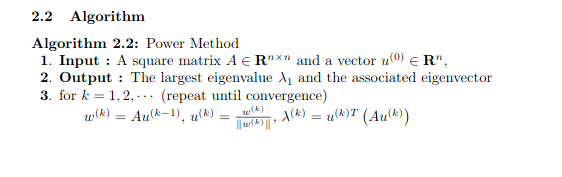
\includegraphics[width=1\linewidth]{images/algoritmo_svd_power_method.png}
\end{center}
\end{figure}

\pagebreak


\section{Implementação e testes - SVD}

\hfill

Implementando um método para obter de decomposição SVD, comparei com o método do numpy np.linalg.svd().

Como medida de comparação, foi gravado o tempo de processamento, e também uma norma erro escolhida.

Essa norma erro foi, dada a matriz original $A$ decomposta, encontrou-se a matriz $A_i^*$, resultante da decomposição, no teste $i$:

\begin{equation}
    \mathlarger{
   A_i^* = \mathcal{U}_i \Sigma_i V_i^T
    }
\end{equation}
obtendo como métrica de desvio $ \epsilon_i = || det(A_i) - det(A_i^*) ||_2$ , e mais genericamente:
\begin{equation}
    \mathlarger{
    \bar{\epsilon} = \frac{1}{K}\sum_{i=1}^{K}(|| det(A_i) - det(A_i^*) ||_2)
    }
\end{equation}

\begin{figure}[H]
\begin{center}
  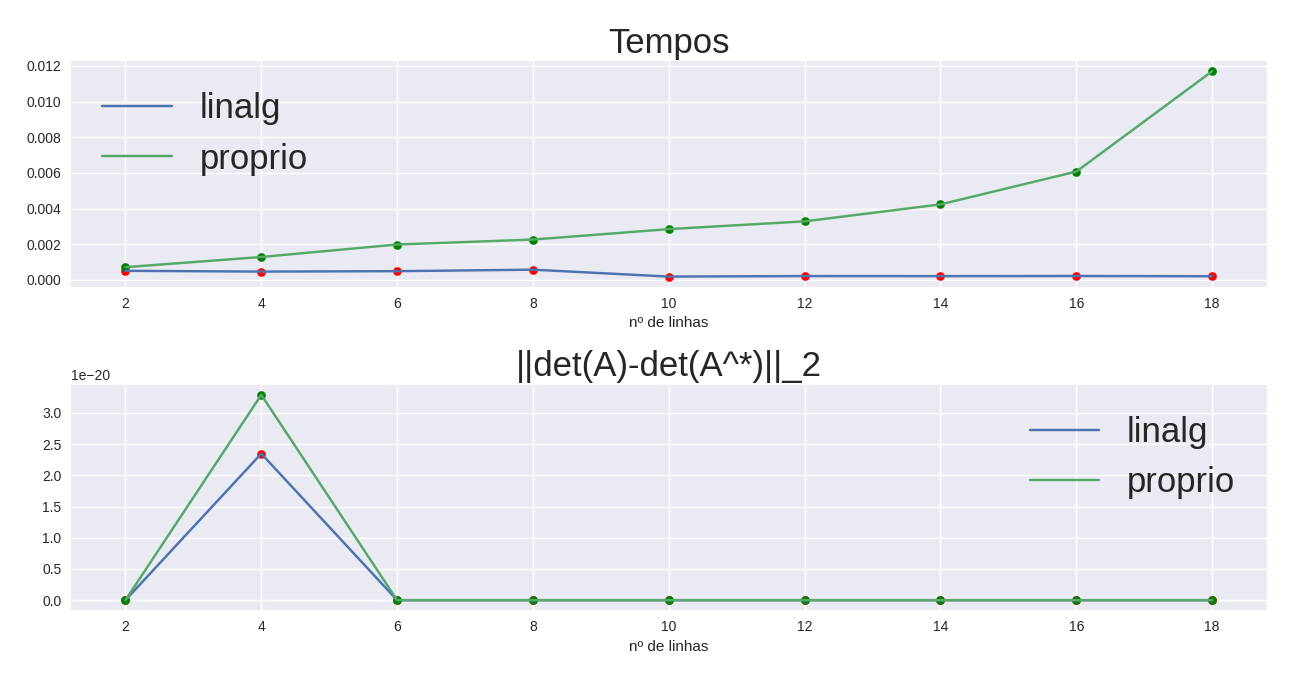
\includegraphics[width=1\linewidth]{images/Figure_1.png}
  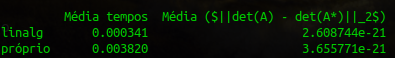
\includegraphics[width=0.6\linewidth]{images/df.png}
\end{center}
\end{figure}

O loop de testes para cada matriz foi implementado utilizando pool de threads como método de paralelismo. Desta maneira, os múltiplos processos de um loop podem ser executados simultaneamente, divididos de acordo com o número de threads e CPUs disponíveis.

As matrizes utilizadas foram geradas de uma sequência de matrizes quadradas, de tamanho múltiplo de 2, e de Hilbert - todo elemento da linha $n$ e coluna $m$ $a_{nm} = \frac{1}{n+m-1}$, no grupo:
\begin{equation}
    \mathlarger{
    \mathcal{M} = \{ A / (a_{nm} = \frac{1}{n+m-1}, \forall a_{nm} \in A) \wedge (n,m \in \{j \}_{j=1}^{K}, K = |A|, K+1 \equiv 1mod(2) )\}
    }
\end{equation}

\pagebreak

\section{Compressão de Imagens - Aplicação do SVD}

\hfill

Por vezes, a compressão de imagens pode ser interessante para reduzir o módulo da quantidade de armazenamento computacional, e está é uma possível aplicação do SVD.

Retornando a matriz resultante da decomposição $\mathcal{U} \Sigma V^T$, mas selecionando uma quantia de componentes:

\hfill


\begin{figure}[!ht]
\begin{center}
  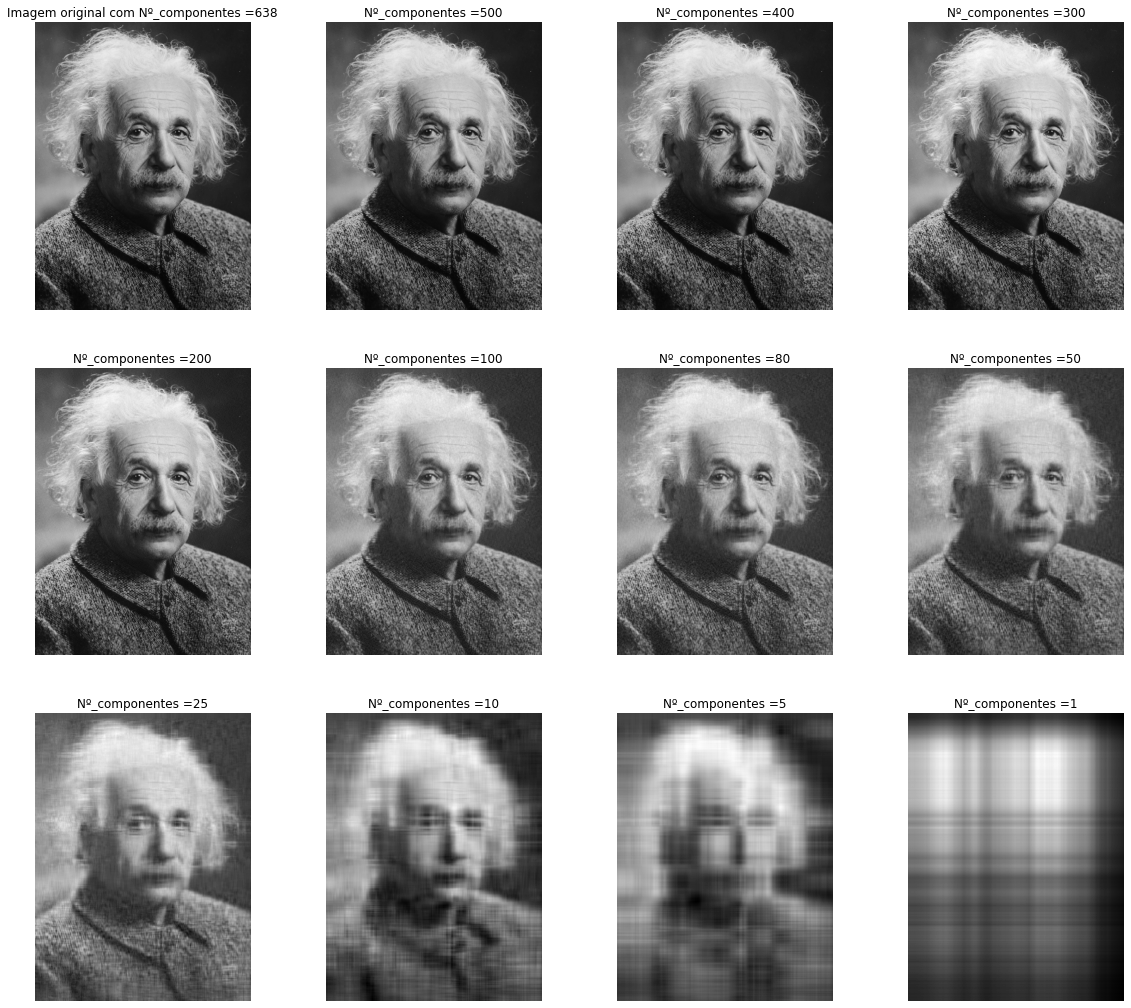
\includegraphics[width=0.85\linewidth]{images/svd_compressao.png}
\end{center}
\end{figure}


\pagebreak

\section{"Auto-faces" (Eigenfaces) - SVD}

\hfill

Primeiramente, vamos recordar que autovetores de uma matriz tem a interpretação de indicarem as direções de máxima variância dos dados. Isto é, a localização da informação mais "relevante".

\begin{equation}
    \mathlarger{
    X \lambda_i = v_i \lambda_i \Rightarrow \{ \lambda_i \}_{i=1}^N,  \{ v_i \}_{i=1}^N
    }
\end{equation}
são, respectivamente, as sequências de autovalores e autovalores da matriz $X$.

Coletados os dados, podem ser encontrados os autovetores associados a cada imagem, exprimindo as direções de máxima variância, e autovalores.

Então, escolhem-se os $K$ maiores autovelores 
\begin{equation}
    \mathlarger{
    \{ || \{ \lambda_i \}_{i=1}^{N-K} ||_{\infty}, ..., || \{ \lambda_i \}_{i=1}^{N} ||_{\infty} \} = \{ || \{ \lambda_i \}_{i=1}^{N-j} ||_{\infty} \}_{j=0}^K
    }
\end{equation}

Então diremos que este conjunto escolhido formará um espaço $S$
\begin{equation}
    \mathlarger{
    || \{ \lambda_i \}_{i=1}^{N-j}||_{\infty} \in S, \forall || \{ \lambda_i \}_{i=1}^{N-j}||_{\infty} \in \{ || \{ \lambda_i \}_{i=1}^{N-j} ||_{\infty} \}_{j=0}^K
    }
\end{equation}

Usaremos este espaço para projetar os dados, encontrando as "faces" mais "próximas", e podemos classificá-las, dicotômicamente, como faces conhecidas ou não.


Utilizando o conjunto de dados \textbf{h lfw people} da biblioteca \textbf{sklearn.datasets} do python:


Após a decomposição SVD
\begin{equation}
    X = \mathcal{U} \Sigma V^T 
\end{equation}

Podemos plotar os valores singulares

\begin{figure}[!ht]
\begin{center}
  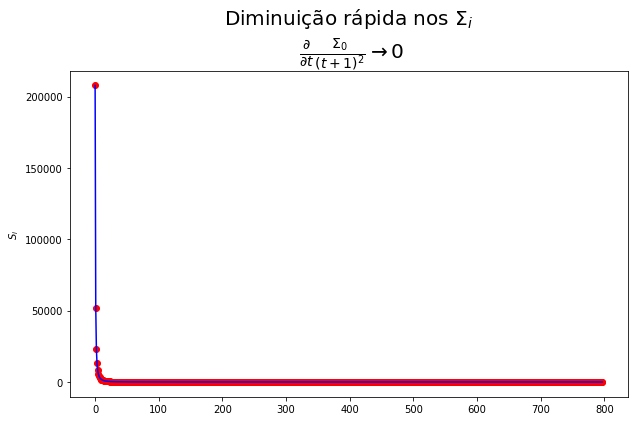
\includegraphics[width=0.45\linewidth]{images/S_decaimento.png}
\end{center}
\end{figure}

E então podemos plotar as "eigenfaces" resultantes:
\begin{figure}[H]
\begin{center}
  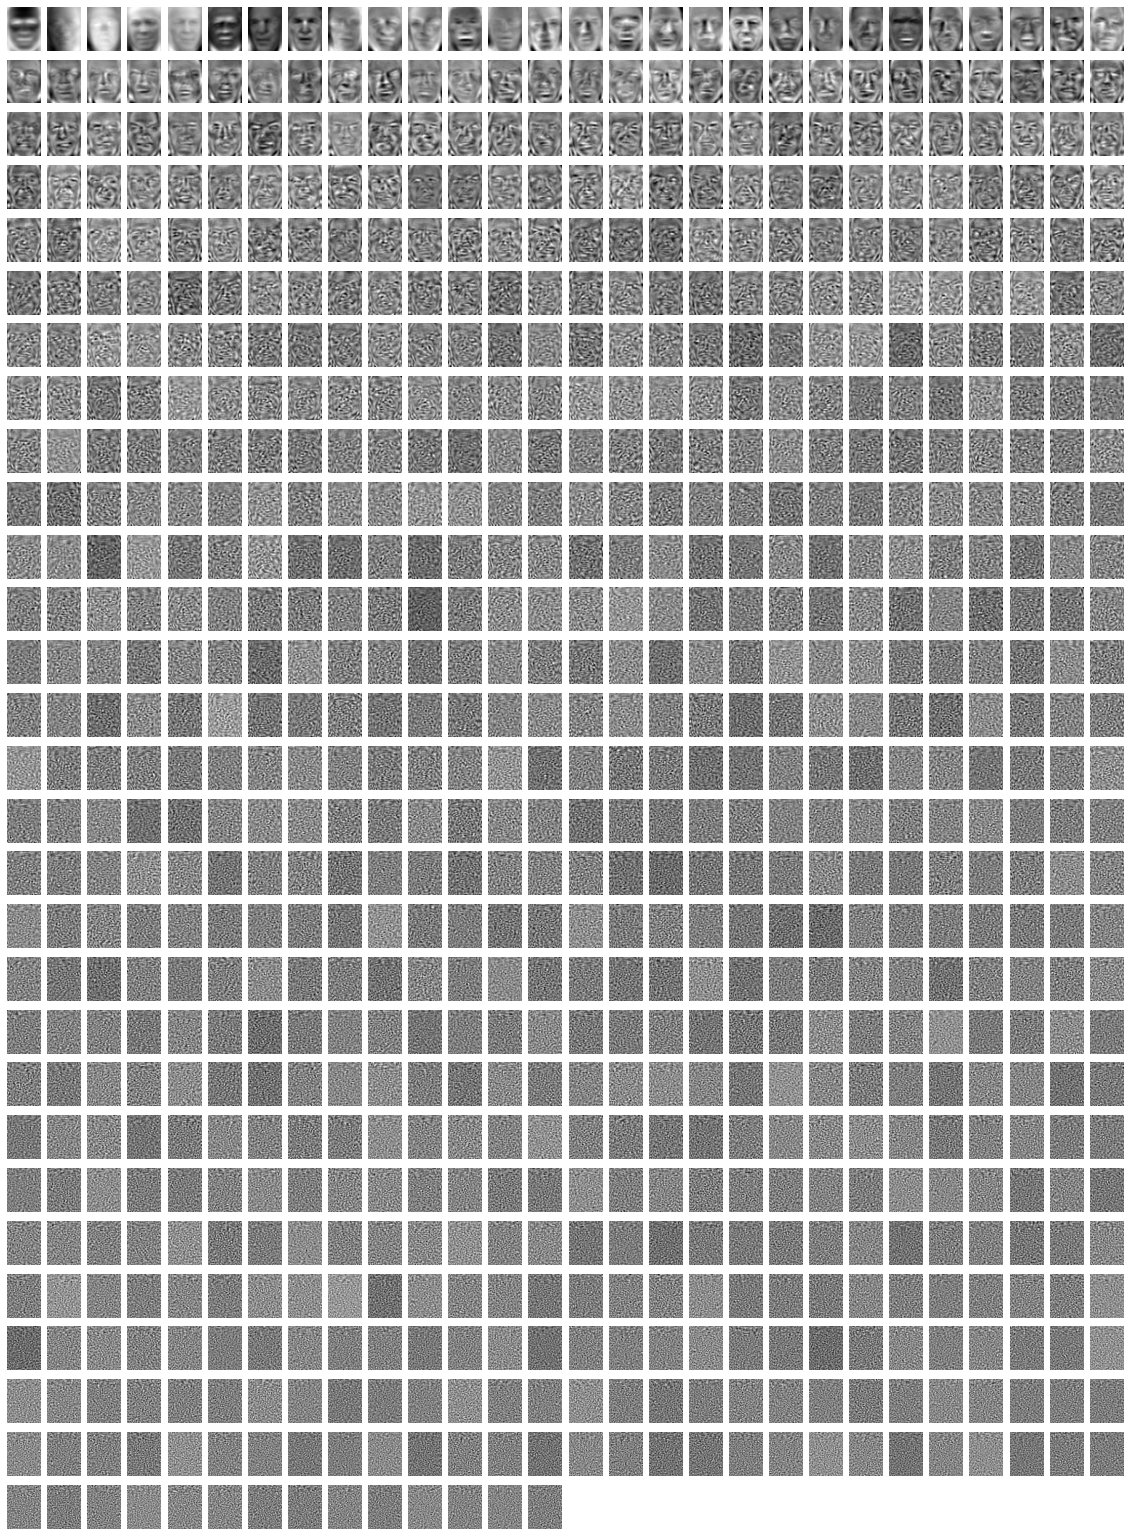
\includegraphics[width=0.4\linewidth]{images/eigenfaces.png}
\end{center}
\end{figure}
\begin{figure}[H]
\begin{center}
  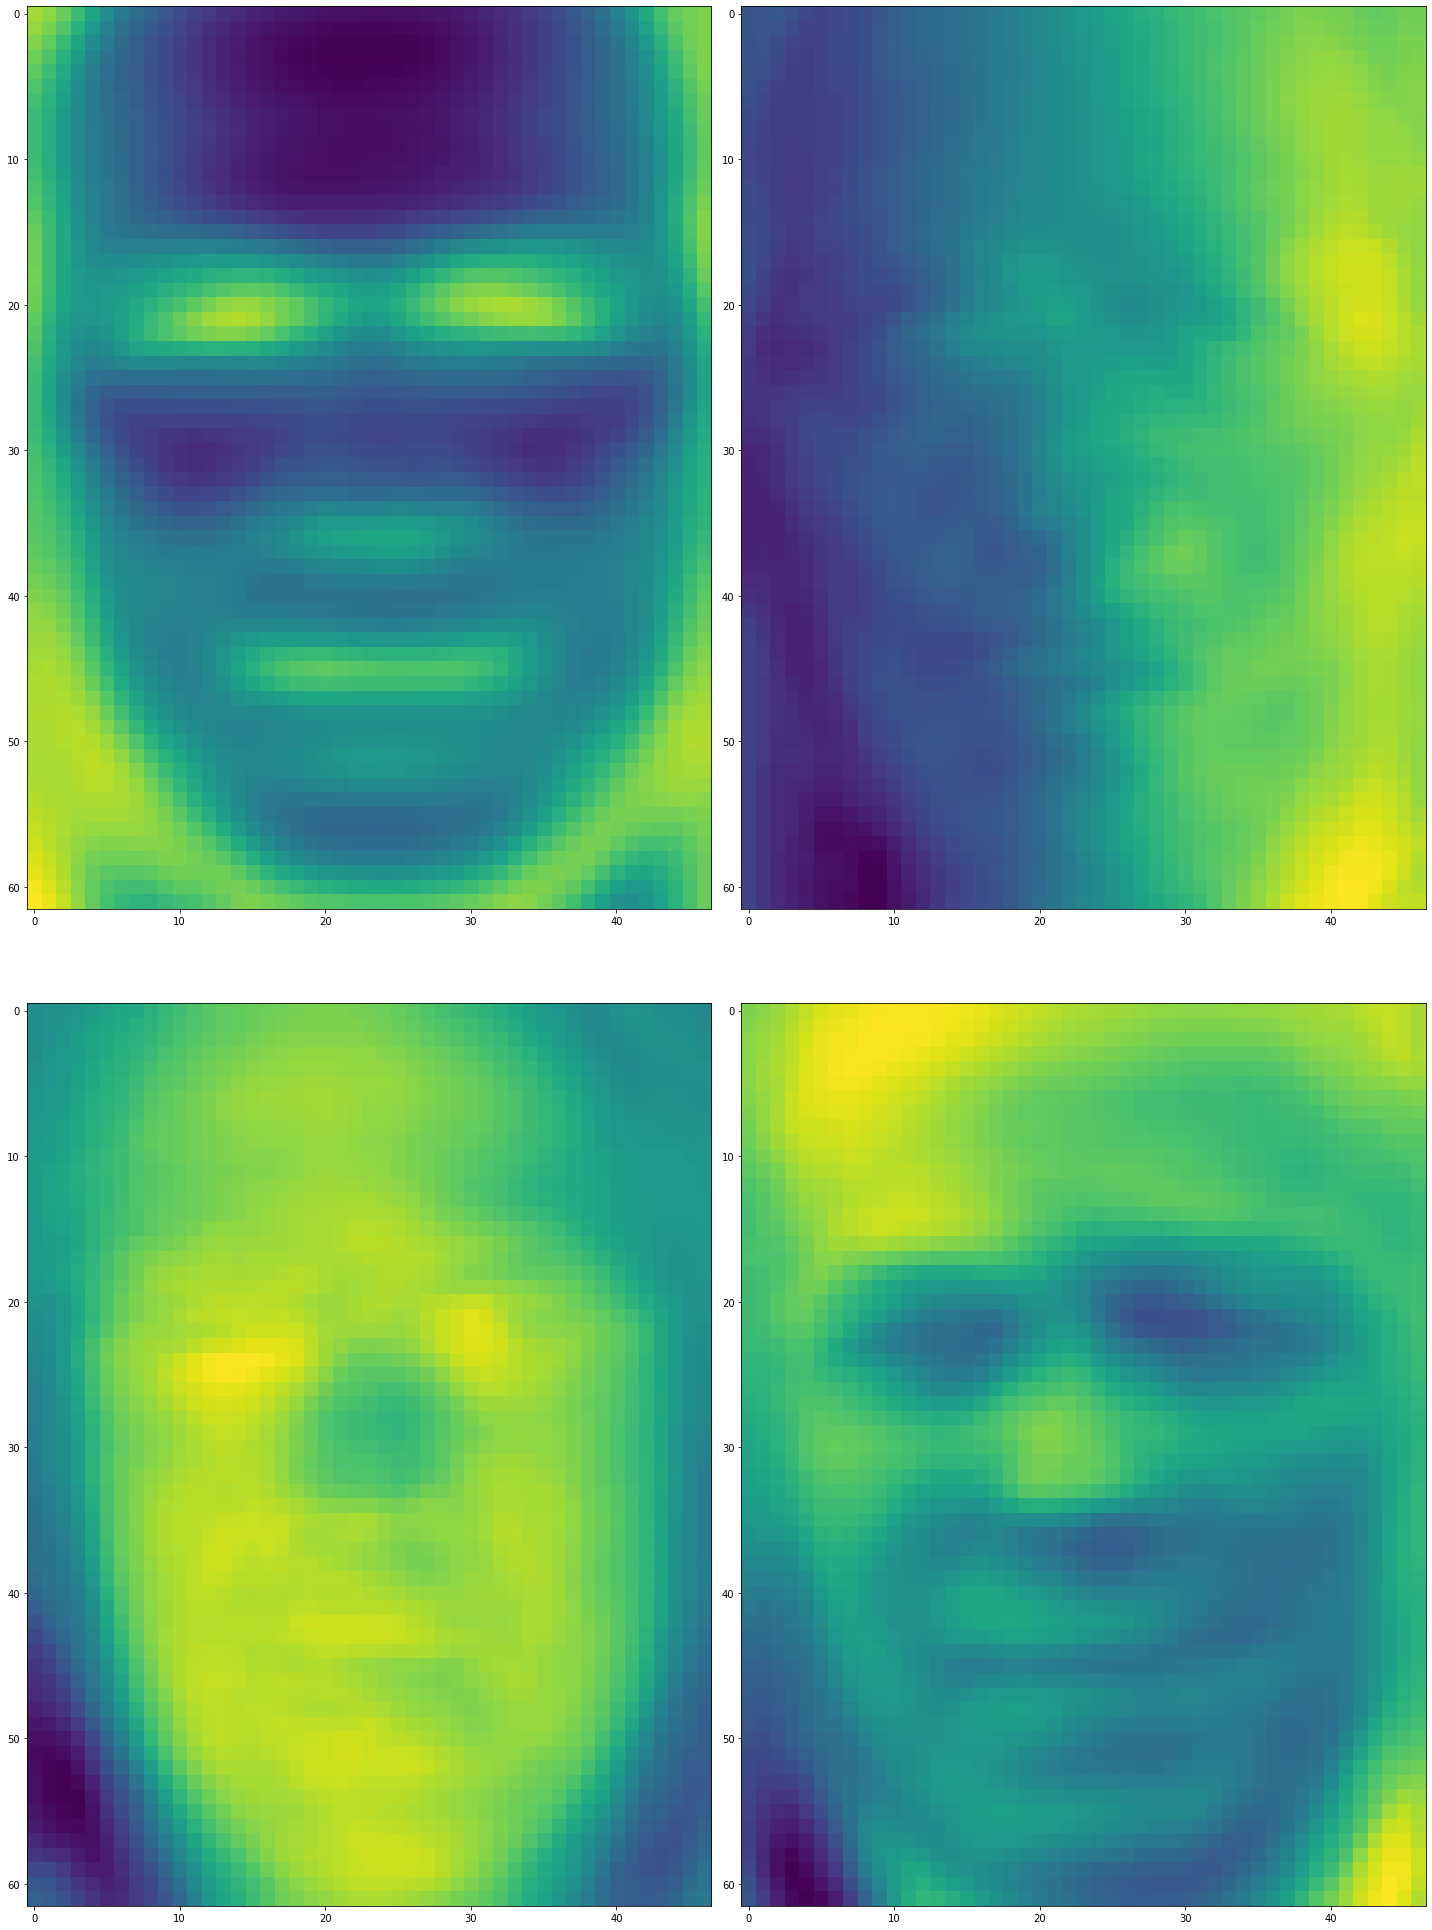
\includegraphics[width=0.3\linewidth]{images/eigenfaces2.png}
\end{center}
\end{figure}

Podemos ver que as imagens expõem características marcantes das faces, em concordância com a hipótese de grande variância dos autovetores.

Em seguida, vamos verificar as imagens no novo espaço:

\begin{figure}[H]
\begin{center}
  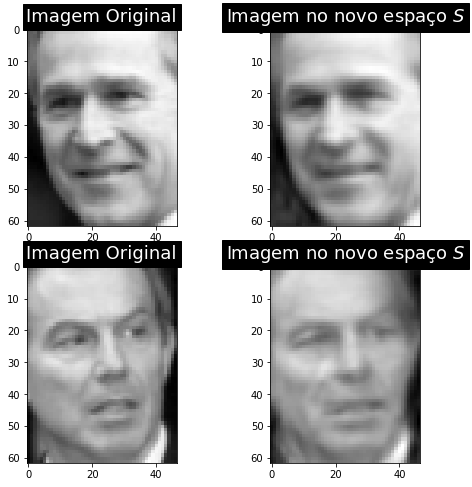
\includegraphics[width=0.4\linewidth]{images/eigenfaces_novo_espaco.png}
\end{center}
\end{figure}


E por fim, podemos aplicar um modelo de classificação para verificar a previsão dos nomes, associados a cada face, no novo espaço.


No caso, apliquei dois modelos: Support Vector Classifier e Random Forest Classifier, para escolher aquele de melhor performance.

Então obtive os resultados:


\begin{figure}[H]
\begin{center}
  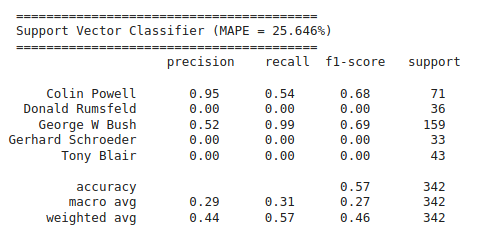
\includegraphics[width=0.45\linewidth]{images/svc.png}
  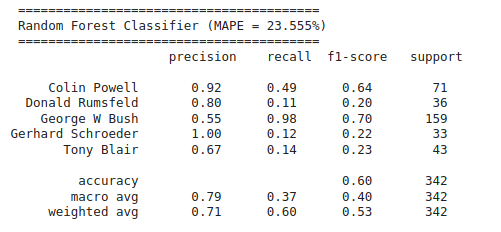
\includegraphics[width=0.45\linewidth]{images/randf.png}
\end{center}
\end{figure}

Comparando os nomes previstos e os reais, para o Random Forest (modelo de menor erro médio percentual:

\begin{figure}[H]
\begin{center}
  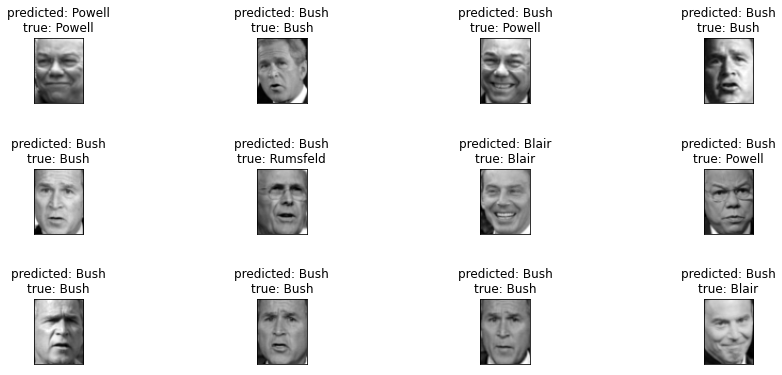
\includegraphics[width=0.65\linewidth]{images/comparacoes_rf.png}
 \end{center}
\end{figure}

Pelo gráfico de variância explicada, vemos a soma cumulativa dos vetores singulares, de acordo com o número de componentes.

\begin{figure}[H]
\begin{center}
  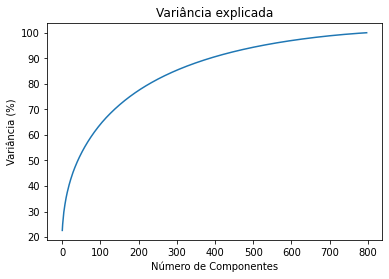
\includegraphics[width=0.45\linewidth]{images/variancia_explicada.png}
\end{center}
\end{figure}


\pagebreak 

\section{Clusterização - Aplicação do PCA}

\hfill

Utilizando o famoso conjunto de dados Iris, com informações de sépalas e pétalas de 3 diferentes espécies de plantas, podemos aplicar a análise de componentes principais a fim de segmentar os dados de acordo com as espécies.


\begin{figure}[ht]
\begin{center}
  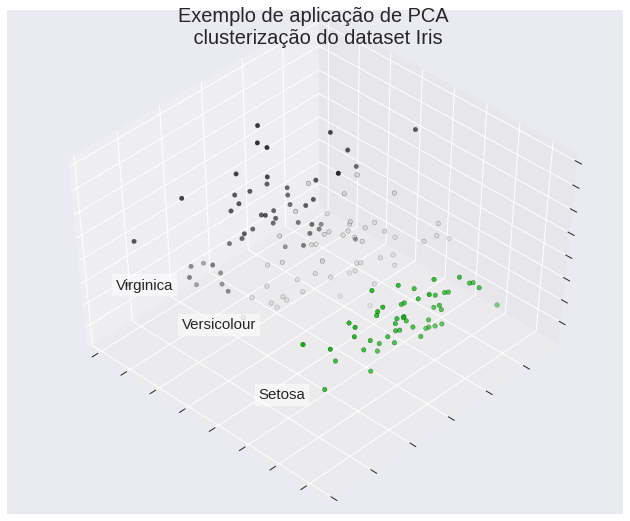
\includegraphics[width=0.6\linewidth]{images/pca_iris.png}
\end{center}
\end{figure}

\pagebreak

\section{Kernel PCA}

\hfill

Neste exemplo, usa-se o Kernel PCA para encontrar uma projeção dos dados, tornando-os linearmente separáveis.

Kernels são amplamente utilizados em algoritmos de classificação e regressão.

Utilizando o exemplo de Support Vector Machines (SVMs), em que, para classificação, os dados são separados linearmente, com bandas (uma faixa acima da reta e outra abaixo, equidistantes da reta, por um tamanho $\epsilon$). Já para regressão, os dados devem ser ajustados entre duas retas, de maneira que maximize o agrupamento dos dados entre as faixas.

Muitas vezes, os dados estão em um espaço em que não são linearmente separáveis. Para atacar este problema, aplica-se uma transformação de espaço, para outro espaço em que um hiperplano gere as bandas.

A partir dos dados $\{ x_j \}_{j=1}^{N}$ e um espaço $S_1$ em que não são linearmente separáveis, faz-se a transformação $\Phi$, passando a sequência para o espaço $S_2$:

\begin{equation}
\mathlarger{
\Phi: S_1 \rightarrow S_2
}
\end{equation}
\begin{equation}
\mathlarger{
\Phi (\{ x_j \}_{j=1}^{N} ) = \{ \hat{x}_j \}_{j=1}^{N}
}
\end{equation}

\begin{figure}[!ht]
\begin{center}
  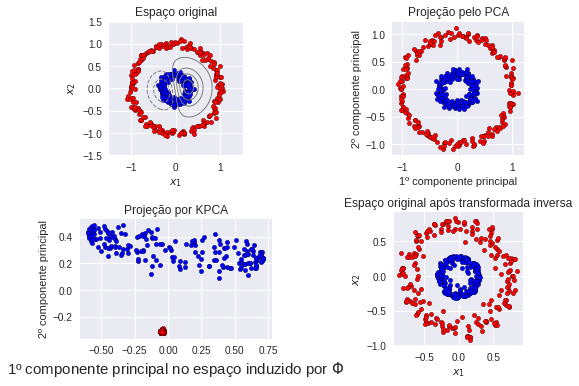
\includegraphics[width=0.8\linewidth]{images/kernel_pca.png}
\end{center}
\end{figure}

\pagebreak

\section{Conceitos importantes}

\hfill

\textbf{Conjugada transposta}

É a transposta da matriz conjugada, obtida pelos conjugados complexos de todos elementos da matriz:

\begin{equation}
\mathlarger{
A_H := \bar{A}^T = \bar{A^T}
}
\end{equation}

\hfill

\textbf{Matriz unitária}
\begin{equation}
\mathlarger{
A A^{-1} = I \text{ , se } A \text{ é uma matriz real}
}
\end{equation}

\textbf{Matriz de Covariância}
Esta quantifica a variabilidade conjunta entre duas variáveis aleatórias $X, Y$ :
\begin{equation}
\mathlarger{
cov(X,Y) = \mathbb{E}[(X -  \mathbb{E}[X])(Y -  \mathbb{E}[Y])]
}
\end{equation}

Vale comentar que caso os valores esperados das duas variáveis aleatórias sejam nulos, a covariância será apenas o produto interno:
\begin{equation}
\mathlarger{
 \mathbb{E}[X] =  \mathbb{E}[Y] = 0 \Rightarrow Cov(X,Y) = \langle X, Y \rangle
}
\end{equation}

Então, a matriz de covariância de uma dada matriz $X$ será:

\begin{equation}
\mathlarger{
C = \frac{\langle X, X \rangle}{n-1} = \frac{ X^T X}{n-1} 
}
\end{equation}


\textbf{Matriz de Rotação}

\begin{equation}
\mathlarger{
M_{\theta} = \begin{pmatrix}
cos \theta & \sin \theta \\
- sin \theta & cos \theta
\end{pmatrix}
}
\end{equation}

Ao multiplicar uma matriz $A$ pela $M_{theta}$ rotaciono as coordenadas de $A$ no ângulo $\theta$.

\hfill


\textbf{Matriz de Hilbert}

Uma matriz $A$ é de Hilbert, se 
\begin{equation}
\mathlarger{
a_{ij} = \frac{1}{i+j-1}, \forall a_{ij} \in A
}
\end{equation}

\pagebreak

\section{Referências Principais}

\hfill

1. Richard L. Burden e J.Douglas Faires. "Numerical Analysis".

2. Strang, Gilbert. "Linear Algebra and its applications".

3. TREVOR, Hastie, TIBSHIRANI, Robert, FRIEDMAN, Jerome, "Elements of Statistical Learning: Data Mining, Inference, and Prediction", 2th edition.

4. sítio https://www.analyticsvidhya.com/blog/2019/08/5-applications-singular-value-decomposition-svd-data-science/

5. sítio https://www.cs.yale.edu/homes/el327/datamining2013aFiles/07_singular_value_decomposition.pdf

6. A. H. Bentbib and A.Kanber, "Block Power Method for SVD Decomposition", http://www.kurims.kyoto-u.ac.jp/EMIS/journals/ASUO/mathematics_/anale2015vol2/Bentbib_A.H.__Kanber_A..pdf

\end{document}
